\documentclass[a4paper, 12pt]{article}
\usepackage[T2A,T1]{fontenc}
\usepackage[utf8]{inputenc}
\usepackage[english, russian]{babel}
\usepackage{graphicx}
\usepackage[hcentering, bindingoffset = 10mm, right = 13 mm, left = 13 mm, top=20mm, bottom = 20 mm]{geometry}
\usepackage{multirow}
\usepackage{lipsum}
\usepackage{amsmath, amstext}
\usepackage{siunitx}
\usepackage{subcaption}
\usepackage{wrapfig}
\usepackage{mathrsfs}
\usepackage{adjustbox}
\usepackage{enumerate, indentfirst, float}
\usepackage{capt-of, svg}
\usepackage{icomma}
\usepackage{xcolor}
\usepackage{ctable}
\usepackage{multirow}

\newenvironment{bottompar}{\par\vspace*{\fill}}{\clearpage}
 
\begin{document}
\begin{titlepage}

\newcommand{\HRule}{\rule{\linewidth}{0.5mm}} % Defines a new command for the horizontal lines, change thickness here

\center % Center everything on the page
 
%----------------------------------------------------------------------------------------
%	HEADING SECTIONS
%----------------------------------------------------------------------------------------

\textsc{\LARGE Московский Физико-Технический Институт}\\[1,5cm] % Name of your university/college
\textsc{\Large Департамент молекулярной и биологической физики}\\[2cm] % Major heading such as course name
\textsc{\large Лабораторная работа}\\[0.5cm] % Minor heading such as course title

%----------------------------------------------------------------------------------------
%	TITLE SECTION
%----------------------------------------------------------------------------------------

\HRule
\\[0.4cm]
{ \huge \bfseries Лиофобные коллоидные растворы}
\\[0.2cm] % Title of your document
\HRule
\\[1.5cm]


 
%----------------------------------------------------------------------------------------
%	AUTHOR SECTION
%----------------------------------------------------------------------------------------
\begin{minipage}{0.4\textwidth}
	\begin{flushleft}		
	\end{flushleft}
\end{minipage}
~
\begin{minipage}{0.4\textwidth}
	\begin{flushright} \large
		\emph{Авторы:}\\
		Светлана \textsc{Фролова} \\
		6113 группа \\
		Анатолий \textsc{Киселёв} \\
		6113 группа
	\end{flushright}
\end{minipage}


\begin{bottompar}
	\begin{center}
		
\includegraphics[width = 80 mm]{logo.jpg}
	\end{center}
	{\large \today}

\end{bottompar}
\vfill % Fill the rest of the page with whitespace

\end{titlepage}

\section{Цели работы}
	\begin{enumerate}
		\item Получить коллоидный раствор золота
		
		\item Определить пороги коагуляции золей с помощью фотометрии
		
		\item Проверить соответствие зависимости порогов коагуляции правилу Дерягина-Ландау
		
	\end{enumerate}
	
\section{Теоретическая часть}
	\subsection*{Типы коллоидных растворов}
	Согласно классификации П. А. Ребиндера коллоидные растворы подразделяются на
лиофильные и лиофобные. Первые, как следует из названия, отличаются большим
сродством к растворителю, диспергированное вещество хорошо смачивается им, а иногда
и набухает в нем. Лиофильные дисперсные системы являются термодинамически
устойчивыми к агрегации и образуются самопроизвольно. К таким системам относятся
растворы гидрофильных полимеров и поверхностно-активных веществ. Зачастую
лиофильные коллоиды сильно увеличивают вязкость растворов. Лиофобные дисперсные
системы, напротив, представляют собой термодинамически неустойчивые к агрегации
системы, образующиеся несамопроизвольно в результате диспергирования или
конденсации с пересыщением. Однако они могут быть устойчивы кинетически.
Лиофобные коллоиды, реагируют с растворителем лишь в незначительной степени, плохо
смачиваются им. Лиофобные дисперсные системы обладают избытком поверхностной
энергии ($G_s = \sigma s$). Поэтому в них самопроизвольно протекают процессы укрупнения
частиц, т. е. происходит снижение поверхностной энергии за счет уменьшения суммарной
площади s частиц дисперсной фазы.

\subsection*{Термодинамические факторы стабилизации коллоидных систем}
Термодинамической устойчивости и самопроизвольному образованию лиофильных
систем отвечает условие
$\Delta G < 0$, или иначе $\Delta H - T\Delta S < 0$\\

В процессе формирования частиц за счет конденсации необходимо пересыщение
раствора, т.к. зародыши малого размера имеют большую растворимость или большее
давление насыщенного пара (для жидкости в газе) за счет высокой кривизны поверхности.
Зависимость давления насыщенного пара от кривизны поверхности определяется
уравнением капиллярной конденсации Кельвина (Томсона):
\[\ln{\frac{p}{p_s} = \frac{\sigma V_M}{RT}\cdot \frac{ds}{dV}} = \frac{2\sigma V_M}{rRT}\]
где $p$ и $p_s$ – давление насыщенного пара над плоской и искривленной поверхностью, $V_M$ –
мольный объем вещества в конденсированном состоянии, $R$ – универсальная газовая
постоянная, $r$ – радиус кривизны зародыша.
Для образования зародыша лиофобной системы требуется энергия на работу по
созданию новой поверхности. Учет этой работы и работы пересыщения дает выражение
для работы образования зародыша:
\[A=-\Delta G=\frac{\sigma S}{3}\]

где $S$ – площадь поверхности зародыша.
\subsection*{Кинетическая устойчивость лиофобных коллоидов}
Как отмечалось выше, устойчивость лиофобных коллоидных систем имеет только
кинетическую природу. Эта агрегативная устойчивость определяется скоростью процесса
коагуляции, который можно описать с помощью уравнения Смолуховского:
\[\nu_\tau = \frac{\nu_0}{1+K\nu_0 \tau}\]
где $\nu_\tau$ – суммарное число частиц дисперсии к времени $\tau$, $\nu_0$ – исходное число частиц, $K$ –
константа скорости коагуляции. Подобно константам скорости химических реакций эта
константа определяется потенциальным барьером при взаимодействии частиц с энергией
активации и стерическим фактором $P$. Кроме этого она существенно зависит от
вязкости растворителя $\eta$:
\[K=\frac{4kT}{3\eta}P\cdot \exp\left(-\frac{\Delta E}{kT}\right)\]
Если в целом константа скорости $K$ определяет медленную (окончательную) коагуляцию,
то первая дробь в последнем выражении (с вязкостью) соответствует константе скорости
$K_\text{б}$ так называемой быстрой коагуляции. При отсутствии энергетического барьера и
стерических затруднений эти величины совпадают и агрегативная устойчивость
коллоидной системы определяется только вязкостью и температурой. В противном случае
система будет более устойчивой к агрегации и фактор устойчивости может быть
охарактеризован величиной $W$:
\[W = \frac{K_\text{б}}{K}=\frac{1}{P}\exp\left(\frac{\Delta E}{kT}\right)\]
При достаточно высоком активационном барьере скорость агрегации может сравняться со
скоростью диспергирования и система окажется устойчивой к коагуляции.

\subsection*{Энергия взаимодействия между частицами в коллоидном растворе}
Согласно теории Гуи-Чапмена толщина двойного электрического слоя (точнее его
диффузной части) известным образом зависит от ионной силы раствора:
\[\lambda=\sqrt{\frac{\varepsilon \varepsilon_0 RT}{2F^2I}}\]
где I – ионная сила раствора.
\[I=\frac{1}{2}\sum{c_iz_i}\]
В соответствии с этими уравнениями, толщина двойного электрического слоя
уменьшается с ростом ионной силы раствора, которая, в свою очередь, наиболее сильно
увеличивается с ростом концентрации многозарядных ионов. Очевидно, что наиболее
эффективно сжимают двойной электрический слой ионы с зарядом того же знака, как и
ионы, создающие его диффузную часть (для отрицательно заряженных частиц – катионы,
а для положительных – анионы), причем многозарядные ионы сжимают двойной
электрический слой наиболее эффективно. Ясно, что при сильном сжатии двойного
электрического слоя практически все противоионы находятся в непосредственном
контакте с заряженной частицей, то есть фактически адсорбированы на ней, и коагуляция
за счет дальнейшего сжатия становится невозможной. В этом случае однозначно сказать о
механизме коагуляции нельзя. По сути, особенно при высоких концентрациях,
задействованы они оба. Описанное влияние электролитов на коагуляцию описывается
правилом Шульце-Гарди: «коагулирующим действием обладают те ионы электролита-
коагулятора, знак заряда которых противоположен заряду частицы дисперсии, а
коагулирующее действие возрастает с увеличением заряда иона-коагулятора. Для одно -
двух и трехвалентного ионов коагулирующее действие примерно относятся как 1: 50: 500.
Касательно механизмов электролитной коагуляции можно сделать вывод, что при
высоких поверхностных зарядах частиц эффективнее проводить концентрационную
коагуляцию (для нейтрализации большого заряда надо слишком много коагулянта), а при
низких – нейтрализационную (небольшой поверхностный заряд легче подавить).\\

Введение электролитов снижает величину
потенциального барьера благодаря увеличению крутизны верхней кривой для
электростатической энергии отталкивания (сжатию двойного слоя), либо уменьшению ее
амплитуды (нейтрализации заряда частицы). Агрегации соответствует исчезновение
потенциального барьера при введении некоторого определенного количества электролита.
Необходимая для этого концентрация электролита называется порогом быстрой
коагуляции $C_{\text{ПК}}$:
\[C_\text{ПК}=C_\text{э}\cdot \frac{V_\text{э}}{V_\text{золь}+V_\text{э}}\]
В соответствии с правилом Дерягина-Ландау при электролитной коагуляции по
концентрационному механизму (который лучше проявляется для сильно заряженных
частиц) порог коагуляции обратно пропорционален заряду противоионов в шестой
степени. Это правило служит теоретическим обоснованием вышеуказанного правила
Шульце-Гарди. Очевидно, концентрационная коагуляция в чистом виде возможна лишь в
достаточно разбавленных растворах электролита, где толщина двойного электрического
слоя достаточно велика.
При нейтрализационной коагуляции (которая проявляется при малых зарядах
поверхности диспергированных частиц) порог коагуляции в соответствии с правилом
Эйлерса-Корфа обратно пропорционален уже лишь второй степени заряда добавляемых
противоионов.



\newpage
\section{Обработка результатов}

\begin{table}[h]
	\centering
	\caption{}
	\label{my-label}
	\begin{tabular}{|l|l|l|l|l|l|l|l|l|l|l|l|l|l|}
\hline
t  & 0     & 10    & 20    & 30    & 40    & 50    & 60    & 70    & 80    & 90    & 100  & 110  & 120  \\ \hline
D & 0,194 & 0,219 & 0,238 & 0,254 & 0,267 & 0,278 & 0,287 & 0,295 & 0,302 & 0,308 & 0,31 & 0,31 & 0,31 \\ \hline
	\end{tabular}
\end{table}

\begin{table}[h]
	\centering
	\caption{}
	\begin{tabular}{|l|l|l|l|}
		\hline
		  &$C_\text{пор} $ & $C_\text{пор, отн} $ & $z^{-6}$ \\ 
		\hline
		$KNO_3$ & $0,016666667$ & $1$ & $1$ \\
		\hline
		$Mg(NO_3)_2$ & $0,000333333$ & $0,02$ &$0,01165$ \\
		\hline
		$La(NO_3)_2$ &$3,33333\cdot 10^{-5}$
 &$0,002$ & $0,00137$ \\
		\hline
	
	\end{tabular}
\end{table}

\begin{figure}[h]
	\centering
	\caption{}
	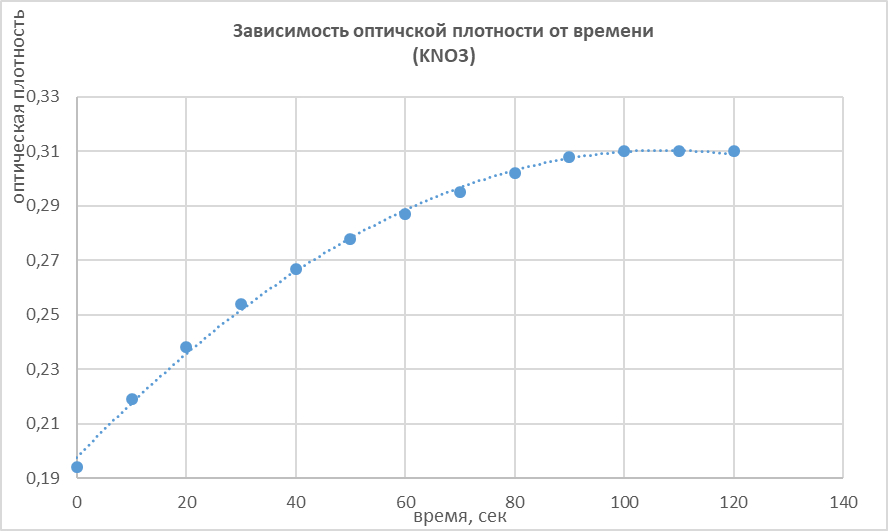
\includegraphics[width=1\textwidth]{image001.png}
\end{figure}
\newpage


\begin{figure}[t]
	\centering
	\caption{}
	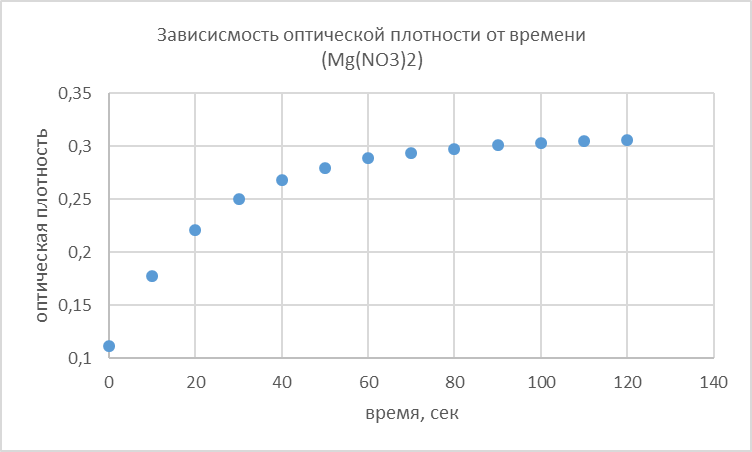
\includegraphics[width=1\textwidth]{image005.png}
\end{figure}

\begin{figure}[h!]
	\centering
	\caption{}
	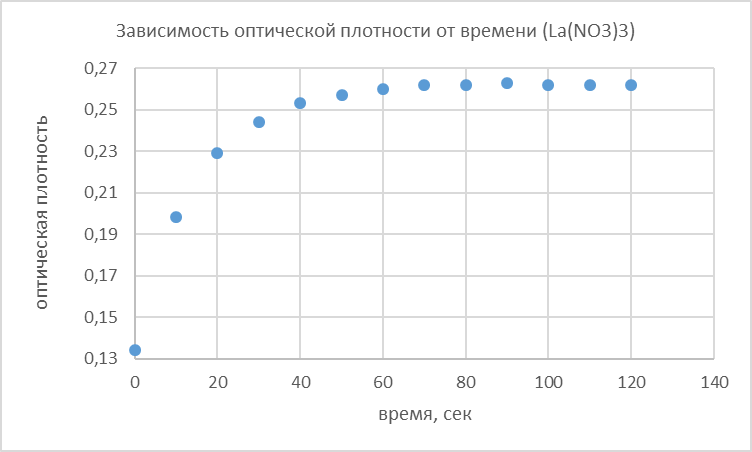
\includegraphics[width=1\textwidth]{image003.png}
\end{figure}

\newpage
\section{Вывод}
Провели серию экспериментов по определению пороговой концентрации коагуляции золей. Получили значения 0,0167 М для нитрата калия, 0,0033 М для нитрата магния и $3,33\cdot10^{-5}$ для нитрата лантана (III). Получили соотношение их концентраций как 1:0,02:0,002, это соответствует закону Дерягина-Ландау, т.е. отношению величин обратно пропорциональных заряду катионов металла в 6-й степени(1:0,01165:0,001373)


\end{document}